\documentclass{standalone}
\usepackage{tikz}
\usepackage{ctex,siunitx}
\usepackage{tkz-euclide}
\usepackage{amsmath}
\usetikzlibrary{patterns, calc}
\usetikzlibrary {decorations.pathmorphing, decorations.pathreplacing, decorations.shapes,}
\begin{document}
\small
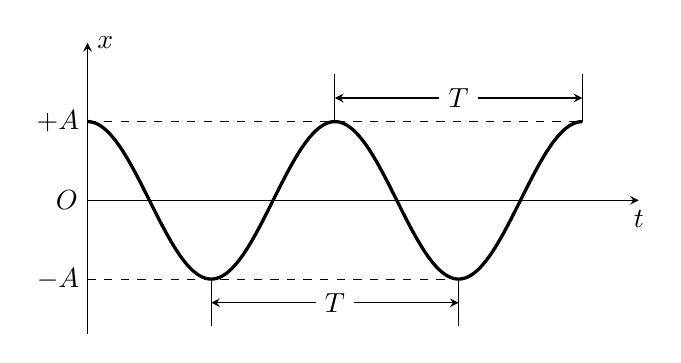
\begin{tikzpicture}[>=stealth,xscale=.5, domain=0:4*pi, samples=200]
  \draw [->](0,0)node [left]{$O$}--(14,0) node [below]{$t$};
  \draw [->](0,-1.7)--(0,2) node [right]{$x$};
  \draw [very thick]  plot (\x,{cos(\x r)});
  \draw [dashed](0, 1) -- (4*pi, 1);  
  \draw [dashed](0,-1) -- (3*pi, -1);     
  \draw[<->](2*pi,1.3)--node[fill=white] {$T$}(4*pi,1.3);
  \draw[<->](pi,-1.3)--node[fill=white] {$T$}(3*pi,-1.3);
  \draw(pi,-1)--(pi,-1.6); \draw(3*pi,-1)--(3*pi,-1.6); 
  \draw(2*pi,1)--(2*pi,1.6); 
  \draw(4*pi,1)--(4*pi,1.6); 
  \node at (-.75,1){$+A$};\node at (-.75,-1){$-A$};
\end{tikzpicture}
\end{document}